% Options for packages loaded elsewhere
% Options for packages loaded elsewhere
\PassOptionsToPackage{unicode}{hyperref}
\PassOptionsToPackage{hyphens}{url}
\PassOptionsToPackage{dvipsnames,svgnames,x11names}{xcolor}
%
\documentclass[
  letterpaper,
  DIV=11,
  numbers=noendperiod]{scrartcl}
\usepackage{xcolor}
\usepackage{amsmath,amssymb}
\setcounter{secnumdepth}{5}
\usepackage{iftex}
\ifPDFTeX
  \usepackage[T1]{fontenc}
  \usepackage[utf8]{inputenc}
  \usepackage{textcomp} % provide euro and other symbols
\else % if luatex or xetex
  \usepackage{unicode-math} % this also loads fontspec
  \defaultfontfeatures{Scale=MatchLowercase}
  \defaultfontfeatures[\rmfamily]{Ligatures=TeX,Scale=1}
\fi
\usepackage{lmodern}
\ifPDFTeX\else
  % xetex/luatex font selection
\fi
% Use upquote if available, for straight quotes in verbatim environments
\IfFileExists{upquote.sty}{\usepackage{upquote}}{}
\IfFileExists{microtype.sty}{% use microtype if available
  \usepackage[]{microtype}
  \UseMicrotypeSet[protrusion]{basicmath} % disable protrusion for tt fonts
}{}
\makeatletter
\@ifundefined{KOMAClassName}{% if non-KOMA class
  \IfFileExists{parskip.sty}{%
    \usepackage{parskip}
  }{% else
    \setlength{\parindent}{0pt}
    \setlength{\parskip}{6pt plus 2pt minus 1pt}}
}{% if KOMA class
  \KOMAoptions{parskip=half}}
\makeatother
% Make \paragraph and \subparagraph free-standing
\makeatletter
\ifx\paragraph\undefined\else
  \let\oldparagraph\paragraph
  \renewcommand{\paragraph}{
    \@ifstar
      \xxxParagraphStar
      \xxxParagraphNoStar
  }
  \newcommand{\xxxParagraphStar}[1]{\oldparagraph*{#1}\mbox{}}
  \newcommand{\xxxParagraphNoStar}[1]{\oldparagraph{#1}\mbox{}}
\fi
\ifx\subparagraph\undefined\else
  \let\oldsubparagraph\subparagraph
  \renewcommand{\subparagraph}{
    \@ifstar
      \xxxSubParagraphStar
      \xxxSubParagraphNoStar
  }
  \newcommand{\xxxSubParagraphStar}[1]{\oldsubparagraph*{#1}\mbox{}}
  \newcommand{\xxxSubParagraphNoStar}[1]{\oldsubparagraph{#1}\mbox{}}
\fi
\makeatother


\usepackage{longtable,booktabs,array}
\newcounter{none} % for unnumbered tables
\usepackage{calc} % for calculating minipage widths
% Correct order of tables after \paragraph or \subparagraph
\usepackage{etoolbox}
\makeatletter
\patchcmd\longtable{\par}{\if@noskipsec\mbox{}\fi\par}{}{}
\makeatother
% Allow footnotes in longtable head/foot
\IfFileExists{footnotehyper.sty}{\usepackage{footnotehyper}}{\usepackage{footnote}}
\makesavenoteenv{longtable}
\usepackage{graphicx}
\makeatletter
\newsavebox\pandoc@box
\newcommand*\pandocbounded[1]{% scales image to fit in text height/width
  \sbox\pandoc@box{#1}%
  \Gscale@div\@tempa{\textheight}{\dimexpr\ht\pandoc@box+\dp\pandoc@box\relax}%
  \Gscale@div\@tempb{\linewidth}{\wd\pandoc@box}%
  \ifdim\@tempb\p@<\@tempa\p@\let\@tempa\@tempb\fi% select the smaller of both
  \ifdim\@tempa\p@<\p@\scalebox{\@tempa}{\usebox\pandoc@box}%
  \else\usebox{\pandoc@box}%
  \fi%
}
% Set default figure placement to htbp
\def\fps@figure{htbp}
\makeatother





\setlength{\emergencystretch}{3em} % prevent overfull lines

\providecommand{\tightlist}{%
  \setlength{\itemsep}{0pt}\setlength{\parskip}{0pt}}



 


\usepackage{array}
\providecommand{\huxb}[2]{\arrayrulecolor[RGB]{#1}\global\arrayrulewidth=#2pt}
\providecommand{\huxvb}[2]{\color[RGB]{#1}\vrule width #2pt}
\providecommand{\huxtpad}[1]{\rule{0pt}{#1}}
\providecommand{\huxbpad}[1]{\rule[-#1]{0pt}{#1}}
\usepackage{caption}
\usepackage{graphicx}
\usepackage{siunitx}
\usepackage[normalem]{ulem}
\usepackage{colortbl}
\usepackage{multirow}
\usepackage{hhline}
\usepackage{calc}
\usepackage{tabularx}
\usepackage{longtable}
\usepackage{threeparttable}
\usepackage{threeparttablex}
\usepackage{wrapfig}
\usepackage{adjustbox}
\usepackage{hyperref}
\KOMAoption{captions}{tableheading,figureheading}
\makeatletter
\@ifpackageloaded{tcolorbox}{}{\usepackage[skins,breakable]{tcolorbox}}
\@ifpackageloaded{fontawesome5}{}{\usepackage{fontawesome5}}
\definecolor{quarto-callout-color}{HTML}{909090}
\definecolor{quarto-callout-note-color}{HTML}{0758E5}
\definecolor{quarto-callout-important-color}{HTML}{CC1914}
\definecolor{quarto-callout-warning-color}{HTML}{EB9113}
\definecolor{quarto-callout-tip-color}{HTML}{00A047}
\definecolor{quarto-callout-caution-color}{HTML}{FC5300}
\definecolor{quarto-callout-color-frame}{HTML}{acacac}
\definecolor{quarto-callout-note-color-frame}{HTML}{4582ec}
\definecolor{quarto-callout-important-color-frame}{HTML}{d9534f}
\definecolor{quarto-callout-warning-color-frame}{HTML}{f0ad4e}
\definecolor{quarto-callout-tip-color-frame}{HTML}{02b875}
\definecolor{quarto-callout-caution-color-frame}{HTML}{fd7e14}
\makeatother
\makeatletter
\@ifpackageloaded{caption}{}{\usepackage{caption}}
\AtBeginDocument{%
\ifdefined\contentsname
  \renewcommand*\contentsname{Table of contents}
\else
  \newcommand\contentsname{Table of contents}
\fi
\ifdefined\listfigurename
  \renewcommand*\listfigurename{List of Figures}
\else
  \newcommand\listfigurename{List of Figures}
\fi
\ifdefined\listtablename
  \renewcommand*\listtablename{List of Tables}
\else
  \newcommand\listtablename{List of Tables}
\fi
\ifdefined\figurename
  \renewcommand*\figurename{Figure}
\else
  \newcommand\figurename{Figure}
\fi
\ifdefined\tablename
  \renewcommand*\tablename{Table}
\else
  \newcommand\tablename{Table}
\fi
}
\@ifpackageloaded{float}{}{\usepackage{float}}
\floatstyle{ruled}
\@ifundefined{c@chapter}{\newfloat{codelisting}{h}{lop}}{\newfloat{codelisting}{h}{lop}[chapter]}
\floatname{codelisting}{Listing}
\newcommand*\listoflistings{\listof{codelisting}{List of Listings}}
\makeatother
\makeatletter
\makeatother
\makeatletter
\@ifpackageloaded{caption}{}{\usepackage{caption}}
\@ifpackageloaded{subcaption}{}{\usepackage{subcaption}}
\makeatother
\usepackage{bookmark}
\IfFileExists{xurl.sty}{\usepackage{xurl}}{} % add URL line breaks if available
\urlstyle{same}
% fallback for those not using the hyperref driver hyperxmp:
\makeatletter
\@ifundefined{xmpquote}{\newcommand{\xmpquote}[1]{#1}}{}
\makeatother
\hypersetup{
  pdftitle={Econometrics 1 --- Problem Set 3},
  pdfauthor={Antonina Wawrzak, David Pérez Cano, Luis Enrique Beltrán González},
  colorlinks=true,
  linkcolor={blue},
  filecolor={Maroon},
  citecolor={Blue},
  urlcolor={Blue},
  pdfcreator={LaTeX via pandoc}}


\title{Econometrics 1 --- Problem Set 3}
\usepackage{etoolbox}
\makeatletter
\providecommand{\subtitle}[1]{% add subtitle to \maketitle
  \apptocmd{\@title}{\par {\large #1 \par}}{}{}
}
\makeatother
\subtitle{Submission Deadline: Thursday, October 15th, 2026 at 1:00 PM
\textbar{} Instructor: Liam Wren-Lewis, TA: Elisa Alonso Herrero}
\author{Antonina Wawrzak, David Pérez Cano, Luis Enrique Beltrán
González}
\date{2026-10-13}
\begin{document}
\maketitle

\renewcommand*\contentsname{Table of contents}
{
\setcounter{tocdepth}{3}
\tableofcontents
}

\subsection{Overview \& Group Work
Division}\label{overview-group-work-division}

\begin{itemize}
\item
  \textbf{Exercise 1 (Theoretical / Reading Critique):}
\item ~
  \subsection{\texorpdfstring{\textbf{Computer Exercise (Empirical
  Analysis in
  R):}}{Computer Exercise (Empirical Analysis in R):}}\label{computer-exercise-empirical-analysis-in-r}
\end{itemize}

\section{Exercise 1: Theoretical \& Reading
Questions}\label{exercise-1-theoretical-reading-questions}

\begin{tcolorbox}[enhanced jigsaw, arc=.35mm, bottomrule=.15mm, bottomtitle=1mm, breakable, colback=white, colbacktitle=quarto-callout-important-color!10!white, colframe=quarto-callout-important-color-frame, coltitle=black, left=2mm, leftrule=.75mm, opacityback=0, opacitybacktitle=0.6, rightrule=.15mm, title=\textcolor{quarto-callout-important-color}{\faExclamation}\hspace{0.5em}{Classmates' Assignment}, titlerule=0mm, toprule=.15mm, toptitle=1mm]

This section contains Exercise 1 (Part A and Part B). Space has been
allocated below for your classmates to fill in their solutions and
write-ups.

\end{tcolorbox}

\subsection{Part A: Article Critique}\label{part-a-article-critique}

\begin{quote}
\textbf{Reading:} \emph{``Legal determinants of World Cup Success''} (by
Mark West).
\end{quote}

\subsubsection{Question 1: Econometric Strategy \& Gauss-Markov
Critique}\label{question-1-econometric-strategy-gauss-markov-critique}

\emph{Formulate a critique related to the econometric strategy used in
the paper. Think about which of the Gauss-Markov assumptions might be
violated in the regressions and what that tells you about the
interpretation of the results. Limit your critique to one page.}

\begin{tcolorbox}[enhanced jigsaw, arc=.35mm, bottomrule=.15mm, bottomtitle=1mm, breakable, colback=white, colbacktitle=quarto-callout-note-color!10!white, colframe=quarto-callout-note-color-frame, coltitle=black, left=2mm, leftrule=.75mm, opacityback=0, opacitybacktitle=0.6, rightrule=.15mm, title=\textcolor{quarto-callout-note-color}{\faInfo}\hspace{0.5em}{Answer --- Exercise 1.A.1}, titlerule=0mm, toprule=.15mm, toptitle=1mm]

\textbf{Violated Gauss-Markov Assumptions \& Implications:}

\begin{itemize}
\item
  \textbf{Zero Conditional Mean Assumption \(E(u|X) = 0\) (Omitted
  Variable Bias):}
\item
  \textbf{Homoskedasticity / Uncorrelated Errors:}
\item
  \textbf{Interpretation of Coefficients:}
\end{itemize}

\end{tcolorbox}

\newpage

\subsubsection{Question 2: Reliability of
Estimations}\label{question-2-reliability-of-estimations}

\emph{The 4 different estimations in this paper seem to lead to quite
different results. If you wanted to conclude anything related to the
determinants of World Cup soccer success, would you rely on any of these
estimations? If so, on which one?}

\begin{tcolorbox}[enhanced jigsaw, arc=.35mm, bottomrule=.15mm, bottomtitle=1mm, breakable, colback=white, colbacktitle=quarto-callout-note-color!10!white, colframe=quarto-callout-note-color-frame, coltitle=black, left=2mm, leftrule=.75mm, opacityback=0, opacitybacktitle=0.6, rightrule=.15mm, title=\textcolor{quarto-callout-note-color}{\faInfo}\hspace{0.5em}{Answer --- Exercise 1.A.2}, titlerule=0mm, toprule=.15mm, toptitle=1mm]

\textbf{Assessment:}

\end{tcolorbox}

\begin{center}\rule{0.5\linewidth}{0.5pt}\end{center}

\subsection{Part B: True or False}\label{part-b-true-or-false}

\emph{Missing observations can lead to both biased estimates and
imprecise estimates. T/F? Explain.}

\begin{tcolorbox}[enhanced jigsaw, arc=.35mm, bottomrule=.15mm, bottomtitle=1mm, breakable, colback=white, colbacktitle=quarto-callout-note-color!10!white, colframe=quarto-callout-note-color-frame, coltitle=black, left=2mm, leftrule=.75mm, opacityback=0, opacitybacktitle=0.6, rightrule=.15mm, title=\textcolor{quarto-callout-note-color}{\faInfo}\hspace{0.5em}{Answer --- Exercise 1.B}, titlerule=0mm, toprule=.15mm, toptitle=1mm]

\textbf{Statement:} \textbf{{[}True / False{]}}

\textbf{Explanation:}

\begin{itemize}
\item
  \textbf{Biased Estimates:}
\item
  \textbf{Imprecise Estimates:}
\end{itemize}

\end{tcolorbox}

\begin{center}\rule{0.5\linewidth}{0.5pt}\end{center}

\section{Computer Exercise: Empirical Analysis in
R}\label{computer-exercise-empirical-analysis-in-r-1}

\begin{tcolorbox}[enhanced jigsaw, arc=.35mm, bottomrule=.15mm, bottomtitle=1mm, breakable, colback=white, colbacktitle=quarto-callout-tip-color!10!white, colframe=quarto-callout-tip-color-frame, coltitle=black, left=2mm, leftrule=.75mm, opacityback=0, opacitybacktitle=0.6, rightrule=.15mm, title=\textcolor{quarto-callout-tip-color}{\faLightbulb}\hspace{0.5em}{Your Assignment}, titlerule=0mm, toprule=.15mm, toptitle=1mm]

This section contains the 7 empirical questions using the dataset
\texttt{nichh.dta}. Code chunks are prepared below for execution in VS
Code / R.

\end{tcolorbox}

\subsection{Data Setup \& Model
Estimation}\label{data-setup-model-estimation}

\begin{quote}
\textbf{Dataset:} \texttt{nichh.dta} (subset of 1998 Nicaragua LSMS
dataset, 582 households).

\textbf{Task:} Estimate a log-linear model that allows understanding the
\emph{ceteris paribus} relationships between total household consumption
(in logs) and household head's age, head's education, male and female
labor endowments, land endowments, and distances to the health clinic
and school.
\end{quote}

\begin{center}\rule{0.5\linewidth}{0.5pt}\end{center}

\subsection{Question (1): Education
Significance}\label{question-1-education-significance}

\emph{What is the minimum significance level at which one can reject the
hypothesis that the education level of the household head does not
affect total household consumption?}

\begin{tcolorbox}[enhanced jigsaw, arc=.35mm, bottomrule=.15mm, bottomtitle=1mm, breakable, colback=white, colbacktitle=quarto-callout-note-color!10!white, colframe=quarto-callout-note-color-frame, coltitle=black, left=2mm, leftrule=.75mm, opacityback=0, opacitybacktitle=0.6, rightrule=.15mm, title=\textcolor{quarto-callout-note-color}{\faInfo}\hspace{0.5em}{Answer --- Question (1)}, titlerule=0mm, toprule=.15mm, toptitle=1mm]

As shown in Table \ref{tbl-model_base_summary}, the coefficient of the
household head's education is statistically significant at the 1\%
significant level, with a p-value of \(<2e-16\) (almost zero). This
means the minimum significance level at which we can reject the null
hypothesis that the education level of the household head does not
affect total household consumption is \(<2e-16\).

\end{tcolorbox}

 
\begin{table}[ht]
\begin{centerbox}
\begin{threeparttable}
\captionsetup{justification=centering,singlelinecheck=off}
\caption{Log-Linear model summary. Dependent variable: log(total household consumption).}
 \label{tbl-model_base_summary}\setlength{\tabcolsep}{0pt}
\begin{tabular}{l l}


\hhline{>{\huxb{0, 0, 0}{0.8}}->{\huxb{0, 0, 0}{0.8}}-}
\arrayrulecolor{black}

\multicolumn{1}{!{\huxvb{0, 0, 0}{0}}c!{\huxvb{0, 0, 0}{0}}}{\huxtpad{1.5pt + 1em}\centering \hspace{1.5pt}  \hspace{1.5pt}\huxbpad{1.5pt}} &
\multicolumn{1}{c!{\huxvb{0, 0, 0}{0}}}{\huxtpad{1.5pt + 1em}\centering \hspace{1.5pt} Log-Linear Model \hspace{1.5pt}\huxbpad{1.5pt}} \tabularnewline[-0.5pt]


\hhline{>{\huxb{255, 255, 255}{0.4}}->{\huxb{0, 0, 0}{0.4}}-}
\arrayrulecolor{black}

\multicolumn{1}{!{\huxvb{0, 0, 0}{0}}l!{\huxvb{0, 0, 0}{0}}}{\huxtpad{1.5pt + 1em}\raggedright \hspace{1.5pt} Intercept \hspace{1.5pt}\huxbpad{1.5pt}} &
\multicolumn{1}{r!{\huxvb{0, 0, 0}{0}}}{\huxtpad{1.5pt + 1em}\raggedleft \hspace{1.5pt} 9.178 *** \hspace{1.5pt}\huxbpad{1.5pt}} \tabularnewline[-0.5pt]


\hhline{}
\arrayrulecolor{black}

\multicolumn{1}{!{\huxvb{0, 0, 0}{0}}l!{\huxvb{0, 0, 0}{0}}}{\huxtpad{1.5pt + 1em}\raggedright \hspace{1.5pt}  \hspace{1.5pt}\huxbpad{1.5pt}} &
\multicolumn{1}{r!{\huxvb{0, 0, 0}{0}}}{\huxtpad{1.5pt + 1em}\raggedleft \hspace{1.5pt} (0.108) [p = 0.000] \hspace{1.5pt}\huxbpad{1.5pt}} \tabularnewline[-0.5pt]


\hhline{}
\arrayrulecolor{black}

\multicolumn{1}{!{\huxvb{0, 0, 0}{0}}l!{\huxvb{0, 0, 0}{0}}}{\huxtpad{1.5pt + 1em}\raggedright \hspace{1.5pt} Number of male adults \hspace{1.5pt}\huxbpad{1.5pt}} &
\multicolumn{1}{r!{\huxvb{0, 0, 0}{0}}}{\huxtpad{1.5pt + 1em}\raggedleft \hspace{1.5pt} 0.115 *** \hspace{1.5pt}\huxbpad{1.5pt}} \tabularnewline[-0.5pt]


\hhline{}
\arrayrulecolor{black}

\multicolumn{1}{!{\huxvb{0, 0, 0}{0}}l!{\huxvb{0, 0, 0}{0}}}{\huxtpad{1.5pt + 1em}\raggedright \hspace{1.5pt}  \hspace{1.5pt}\huxbpad{1.5pt}} &
\multicolumn{1}{r!{\huxvb{0, 0, 0}{0}}}{\huxtpad{1.5pt + 1em}\raggedleft \hspace{1.5pt} (0.025) [p = 0.000] \hspace{1.5pt}\huxbpad{1.5pt}} \tabularnewline[-0.5pt]


\hhline{}
\arrayrulecolor{black}

\multicolumn{1}{!{\huxvb{0, 0, 0}{0}}l!{\huxvb{0, 0, 0}{0}}}{\huxtpad{1.5pt + 1em}\raggedright \hspace{1.5pt} Number of female adults \hspace{1.5pt}\huxbpad{1.5pt}} &
\multicolumn{1}{r!{\huxvb{0, 0, 0}{0}}}{\huxtpad{1.5pt + 1em}\raggedleft \hspace{1.5pt} 0.195 *** \hspace{1.5pt}\huxbpad{1.5pt}} \tabularnewline[-0.5pt]


\hhline{}
\arrayrulecolor{black}

\multicolumn{1}{!{\huxvb{0, 0, 0}{0}}l!{\huxvb{0, 0, 0}{0}}}{\huxtpad{1.5pt + 1em}\raggedright \hspace{1.5pt}  \hspace{1.5pt}\huxbpad{1.5pt}} &
\multicolumn{1}{r!{\huxvb{0, 0, 0}{0}}}{\huxtpad{1.5pt + 1em}\raggedleft \hspace{1.5pt} (0.025) [p = 0.000] \hspace{1.5pt}\huxbpad{1.5pt}} \tabularnewline[-0.5pt]


\hhline{}
\arrayrulecolor{black}

\multicolumn{1}{!{\huxvb{0, 0, 0}{0}}l!{\huxvb{0, 0, 0}{0}}}{\huxtpad{1.5pt + 1em}\raggedright \hspace{1.5pt} Age of household head (years) \hspace{1.5pt}\huxbpad{1.5pt}} &
\multicolumn{1}{r!{\huxvb{0, 0, 0}{0}}}{\huxtpad{1.5pt + 1em}\raggedleft \hspace{1.5pt} 0.006 *** \hspace{1.5pt}\huxbpad{1.5pt}} \tabularnewline[-0.5pt]


\hhline{}
\arrayrulecolor{black}

\multicolumn{1}{!{\huxvb{0, 0, 0}{0}}l!{\huxvb{0, 0, 0}{0}}}{\huxtpad{1.5pt + 1em}\raggedright \hspace{1.5pt}  \hspace{1.5pt}\huxbpad{1.5pt}} &
\multicolumn{1}{r!{\huxvb{0, 0, 0}{0}}}{\huxtpad{1.5pt + 1em}\raggedleft \hspace{1.5pt} (0.002) [p = 0.000] \hspace{1.5pt}\huxbpad{1.5pt}} \tabularnewline[-0.5pt]


\hhline{}
\arrayrulecolor{black}

\multicolumn{1}{!{\huxvb{0, 0, 0}{0}}l!{\huxvb{0, 0, 0}{0}}}{\huxtpad{1.5pt + 1em}\raggedright \hspace{1.5pt} Education of household head (years) \hspace{1.5pt}\huxbpad{1.5pt}} &
\multicolumn{1}{r!{\huxvb{0, 0, 0}{0}}}{\huxtpad{1.5pt + 1em}\raggedleft \hspace{1.5pt} 0.066 *** \hspace{1.5pt}\huxbpad{1.5pt}} \tabularnewline[-0.5pt]


\hhline{}
\arrayrulecolor{black}

\multicolumn{1}{!{\huxvb{0, 0, 0}{0}}l!{\huxvb{0, 0, 0}{0}}}{\huxtpad{1.5pt + 1em}\raggedright \hspace{1.5pt}  \hspace{1.5pt}\huxbpad{1.5pt}} &
\multicolumn{1}{r!{\huxvb{0, 0, 0}{0}}}{\huxtpad{1.5pt + 1em}\raggedleft \hspace{1.5pt} (0.005) [p = 0.000] \hspace{1.5pt}\huxbpad{1.5pt}} \tabularnewline[-0.5pt]


\hhline{}
\arrayrulecolor{black}

\multicolumn{1}{!{\huxvb{0, 0, 0}{0}}l!{\huxvb{0, 0, 0}{0}}}{\huxtpad{1.5pt + 1em}\raggedright \hspace{1.5pt} Land owned (ha) \hspace{1.5pt}\huxbpad{1.5pt}} &
\multicolumn{1}{r!{\huxvb{0, 0, 0}{0}}}{\huxtpad{1.5pt + 1em}\raggedleft \hspace{1.5pt} 0.004 *** \hspace{1.5pt}\huxbpad{1.5pt}} \tabularnewline[-0.5pt]


\hhline{}
\arrayrulecolor{black}

\multicolumn{1}{!{\huxvb{0, 0, 0}{0}}l!{\huxvb{0, 0, 0}{0}}}{\huxtpad{1.5pt + 1em}\raggedright \hspace{1.5pt}  \hspace{1.5pt}\huxbpad{1.5pt}} &
\multicolumn{1}{r!{\huxvb{0, 0, 0}{0}}}{\huxtpad{1.5pt + 1em}\raggedleft \hspace{1.5pt} (0.001) [p = 0.000] \hspace{1.5pt}\huxbpad{1.5pt}} \tabularnewline[-0.5pt]


\hhline{}
\arrayrulecolor{black}

\multicolumn{1}{!{\huxvb{0, 0, 0}{0}}l!{\huxvb{0, 0, 0}{0}}}{\huxtpad{1.5pt + 1em}\raggedright \hspace{1.5pt} Distance to health centre (km) \hspace{1.5pt}\huxbpad{1.5pt}} &
\multicolumn{1}{r!{\huxvb{0, 0, 0}{0}}}{\huxtpad{1.5pt + 1em}\raggedleft \hspace{1.5pt} -0.011 \hspace{1.5pt}\huxbpad{1.5pt}} \tabularnewline[-0.5pt]


\hhline{}
\arrayrulecolor{black}

\multicolumn{1}{!{\huxvb{0, 0, 0}{0}}l!{\huxvb{0, 0, 0}{0}}}{\huxtpad{1.5pt + 1em}\raggedright \hspace{1.5pt}  \hspace{1.5pt}\huxbpad{1.5pt}} &
\multicolumn{1}{r!{\huxvb{0, 0, 0}{0}}}{\huxtpad{1.5pt + 1em}\raggedleft \hspace{1.5pt} (0.010) [p = 0.294] \hspace{1.5pt}\huxbpad{1.5pt}} \tabularnewline[-0.5pt]


\hhline{}
\arrayrulecolor{black}

\multicolumn{1}{!{\huxvb{0, 0, 0}{0}}l!{\huxvb{0, 0, 0}{0}}}{\huxtpad{1.5pt + 1em}\raggedright \hspace{1.5pt} Distance to school (km) \hspace{1.5pt}\huxbpad{1.5pt}} &
\multicolumn{1}{r!{\huxvb{0, 0, 0}{0}}}{\huxtpad{1.5pt + 1em}\raggedleft \hspace{1.5pt} -0.020 * \hspace{1.5pt}\huxbpad{1.5pt}} \tabularnewline[-0.5pt]


\hhline{}
\arrayrulecolor{black}

\multicolumn{1}{!{\huxvb{0, 0, 0}{0}}l!{\huxvb{0, 0, 0}{0}}}{\huxtpad{1.5pt + 1em}\raggedright \hspace{1.5pt}  \hspace{1.5pt}\huxbpad{1.5pt}} &
\multicolumn{1}{r!{\huxvb{0, 0, 0}{0}}}{\huxtpad{1.5pt + 1em}\raggedleft \hspace{1.5pt} (0.011) [p = 0.080] \hspace{1.5pt}\huxbpad{1.5pt}} \tabularnewline[-0.5pt]


\hhline{>{\huxb{255, 255, 255}{0.4}}->{\huxb{0, 0, 0}{0.4}}-}
\arrayrulecolor{black}

\multicolumn{1}{!{\huxvb{0, 0, 0}{0}}l!{\huxvb{0, 0, 0}{0}}}{\huxtpad{1.5pt + 1em}\raggedright \hspace{1.5pt} N \hspace{1.5pt}\huxbpad{1.5pt}} &
\multicolumn{1}{r!{\huxvb{0, 0, 0}{0}}}{\huxtpad{1.5pt + 1em}\raggedleft \hspace{1.5pt} 575 \hspace{1.5pt}\huxbpad{1.5pt}} \tabularnewline[-0.5pt]


\hhline{}
\arrayrulecolor{black}

\multicolumn{1}{!{\huxvb{0, 0, 0}{0}}l!{\huxvb{0, 0, 0}{0}}}{\huxtpad{1.5pt + 1em}\raggedright \hspace{1.5pt} R2 \hspace{1.5pt}\huxbpad{1.5pt}} &
\multicolumn{1}{r!{\huxvb{0, 0, 0}{0}}}{\huxtpad{1.5pt + 1em}\raggedleft \hspace{1.5pt} 0.354 \hspace{1.5pt}\huxbpad{1.5pt}} \tabularnewline[-0.5pt]


\hhline{>{\huxb{0, 0, 0}{0.8}}->{\huxb{0, 0, 0}{0.8}}-}
\arrayrulecolor{black}
\end{tabular}
\begin{tablenotes}[flushleft]
\item[] Significance: *** p $<$ 0.01; ** p $<$ 0.05; * p $<$ 0.1
\end{tablenotes}
\end{threeparttable}\par\end{centerbox}

\end{table}
 

\begin{center}\rule{0.5\linewidth}{0.5pt}\end{center}

\subsection{Question (2): Male vs.~Female Labor
Returns}\label{question-2-male-vs.-female-labor-returns}

\emph{Do your results allow you to conclude the returns to male adults
in the household are larger than the returns to female adults? State the
null hypothesis and the alternative hypothesis you are testing, and the
significance level you are considering. Do the test and discuss. Does
your answer differ depending on which significance level you consider?}

\begin{tcolorbox}[enhanced jigsaw, arc=.35mm, bottomrule=.15mm, bottomtitle=1mm, breakable, colback=white, colbacktitle=quarto-callout-note-color!10!white, colframe=quarto-callout-note-color-frame, coltitle=black, left=2mm, leftrule=.75mm, opacityback=0, opacitybacktitle=0.6, rightrule=.15mm, title=\textcolor{quarto-callout-note-color}{\faInfo}\hspace{0.5em}{Answer --- Question (2)}, titlerule=0mm, toprule=.15mm, toptitle=1mm]

Recalling the model functional form: \[
\begin{aligned}
\label{eq:functional_form}
\log(\text{ConsTotal}) & = \beta_0 + \beta_1 \text{Adult}_{Male} + \beta_2 \text{Adult}_{Female} + \text{C} \text{Z} + u
& \text{Where } \text{Z} \text{ represents the vector of control variables and C is the vector of their coefficients.} 
\end{aligned}
\]

Using Equation \ref{eq:functional_form} the null and alternative
hypotheses are as follows:

\[
\begin{aligned}
H_0: & \beta_1 \leq \beta_2 \\
H_1: & \beta_1 > \beta_2
\end{aligned}
\]

\begin{verbatim}
   adultm 
-2.090923 
\end{verbatim}

Running a one sided t-test to verify that \(\beta_1 - \beta_2 > 0\), the
results show a t-statistic of \(-2.090923\) which \(t\) is less than any
critical value for the significance levels of 1\%, 5\%, or 10\%. In
fact, for one sided tests any t-statistic less than zero will fail to
reject the null hypothesis because its p-value will be greater than the
significance level. Therefore, we can not conclude that returns to male
adults in the household are larger than the returns to female adults
regardless of the significance level considered.

\end{tcolorbox}

\begin{center}\rule{0.5\linewidth}{0.5pt}\end{center}

\subsection{Question (3): Joint Significance of Distance
Variables}\label{question-3-joint-significance-of-distance-variables}

\emph{Test whether the 2 distance variables are jointly significant.
Calculate the test by hand (using R). What can you conclude about the
role of isolation on household welfare?}

\begin{tcolorbox}[enhanced jigsaw, arc=.35mm, bottomrule=.15mm, bottomtitle=1mm, breakable, colback=white, colbacktitle=quarto-callout-note-color!10!white, colframe=quarto-callout-note-color-frame, coltitle=black, left=2mm, leftrule=.75mm, opacityback=0, opacitybacktitle=0.6, rightrule=.15mm, title=\textcolor{quarto-callout-note-color}{\faInfo}\hspace{0.5em}{Answer --- Question (3)}, titlerule=0mm, toprule=.15mm, toptitle=1mm]

Let's estimate the restricted and unrestricted models and calculate the
F-statistic by hand:

\begin{verbatim}
[1] 2.593946
\end{verbatim}

\begin{verbatim}
[1] 2.311961
\end{verbatim}

Using the standard formula for the F-statistic: \[
\begin{aligned}
F &= \frac{(RSS_R - RSS_U) / q}{RSS_U / (n - k - 1)}\\
& = \frac{(192.4492-190.7043)/2}{190.7043/(575-7-1)} = 2.59
\end{aligned}
\]

Since the critical value for the F-distribution with 2 restrictions and
567 degrees of freedom is 3.01, we fail to reject the null hypothesis
that the two distance variables are jointly insignificant. However, we
can reject the null hypothesis at a 10\% significance level, as the
critical value for that level is 2.31. This suggest that isolation
(measured by distance to health clinic and school) has a weak but
significant effect on household welfare, and that the two distance
variables are jointly significant at a 10\% significance level.

\end{tcolorbox}

\begin{center}\rule{0.5\linewidth}{0.5pt}\end{center}

\subsection{Question (4): Correlation Between Education and
Age}\label{question-4-correlation-between-education-and-age}

\emph{Analyze the correlation between households' education and age.
What does this correlation imply for your estimates? If you are
estimating this model to obtain an estimate of the returns to
household's heads education on household welfare, should you keep
household age in the model?}

\begin{tcolorbox}[enhanced jigsaw, arc=.35mm, bottomrule=.15mm, bottomtitle=1mm, breakable, colback=white, colbacktitle=quarto-callout-note-color!10!white, colframe=quarto-callout-note-color-frame, coltitle=black, left=2mm, leftrule=.75mm, opacityback=0, opacitybacktitle=0.6, rightrule=.15mm, title=\textcolor{quarto-callout-note-color}{\faInfo}\hspace{0.5em}{Answer --- Question (4)}, titlerule=0mm, toprule=.15mm, toptitle=1mm]

\end{tcolorbox}

\begin{verbatim}
[1] -0.3117732
\end{verbatim}

 
\begin{table}[ht]
\begin{centerbox}
\begin{threeparttable}
\setlength{\tabcolsep}{0pt}
\begin{tabular}{l l l}


\hhline{>{\huxb{0, 0, 0}{0.8}}->{\huxb{0, 0, 0}{0.8}}->{\huxb{0, 0, 0}{0.8}}-}
\arrayrulecolor{black}

\multicolumn{1}{!{\huxvb{0, 0, 0}{0}}c!{\huxvb{0, 0, 0}{0}}}{\huxtpad{6pt + 1em}\centering \hspace{6pt}  \hspace{6pt}\huxbpad{6pt}} &
\multicolumn{1}{c!{\huxvb{0, 0, 0}{0}}}{\huxtpad{6pt + 1em}\centering \hspace{6pt} Model with Age \hspace{6pt}\huxbpad{6pt}} &
\multicolumn{1}{c!{\huxvb{0, 0, 0}{0}}}{\huxtpad{6pt + 1em}\centering \hspace{6pt} Model without Age \hspace{6pt}\huxbpad{6pt}} \tabularnewline[-0.5pt]


\hhline{>{\huxb{255, 255, 255}{0.4}}->{\huxb{0, 0, 0}{0.4}}->{\huxb{0, 0, 0}{0.4}}-}
\arrayrulecolor{black}

\multicolumn{1}{!{\huxvb{0, 0, 0}{0}}l!{\huxvb{0, 0, 0}{0}}}{\huxtpad{6pt + 1em}\raggedright \hspace{6pt} Intercept \hspace{6pt}\huxbpad{6pt}} &
\multicolumn{1}{r!{\huxvb{0, 0, 0}{0}}}{\huxtpad{6pt + 1em}\raggedleft \hspace{6pt} 9.178 *** \hspace{6pt}\huxbpad{6pt}} &
\multicolumn{1}{r!{\huxvb{0, 0, 0}{0}}}{\huxtpad{6pt + 1em}\raggedleft \hspace{6pt} 9.470 *** \hspace{6pt}\huxbpad{6pt}} \tabularnewline[-0.5pt]


\hhline{}
\arrayrulecolor{black}

\multicolumn{1}{!{\huxvb{0, 0, 0}{0}}l!{\huxvb{0, 0, 0}{0}}}{\huxtpad{6pt + 1em}\raggedright \hspace{6pt}  \hspace{6pt}\huxbpad{6pt}} &
\multicolumn{1}{r!{\huxvb{0, 0, 0}{0}}}{\huxtpad{6pt + 1em}\raggedleft \hspace{6pt} (0.108) \hspace{6pt}\huxbpad{6pt}} &
\multicolumn{1}{r!{\huxvb{0, 0, 0}{0}}}{\huxtpad{6pt + 1em}\raggedleft \hspace{6pt} (0.076) \hspace{6pt}\huxbpad{6pt}} \tabularnewline[-0.5pt]


\hhline{}
\arrayrulecolor{black}

\multicolumn{1}{!{\huxvb{0, 0, 0}{0}}l!{\huxvb{0, 0, 0}{0}}}{\huxtpad{6pt + 1em}\raggedright \hspace{6pt} Number of male adults \hspace{6pt}\huxbpad{6pt}} &
\multicolumn{1}{r!{\huxvb{0, 0, 0}{0}}}{\huxtpad{6pt + 1em}\raggedleft \hspace{6pt} 0.115 *** \hspace{6pt}\huxbpad{6pt}} &
\multicolumn{1}{r!{\huxvb{0, 0, 0}{0}}}{\huxtpad{6pt + 1em}\raggedleft \hspace{6pt} 0.126 *** \hspace{6pt}\huxbpad{6pt}} \tabularnewline[-0.5pt]


\hhline{}
\arrayrulecolor{black}

\multicolumn{1}{!{\huxvb{0, 0, 0}{0}}l!{\huxvb{0, 0, 0}{0}}}{\huxtpad{6pt + 1em}\raggedright \hspace{6pt}  \hspace{6pt}\huxbpad{6pt}} &
\multicolumn{1}{r!{\huxvb{0, 0, 0}{0}}}{\huxtpad{6pt + 1em}\raggedleft \hspace{6pt} (0.025) \hspace{6pt}\huxbpad{6pt}} &
\multicolumn{1}{r!{\huxvb{0, 0, 0}{0}}}{\huxtpad{6pt + 1em}\raggedleft \hspace{6pt} (0.025) \hspace{6pt}\huxbpad{6pt}} \tabularnewline[-0.5pt]


\hhline{}
\arrayrulecolor{black}

\multicolumn{1}{!{\huxvb{0, 0, 0}{0}}l!{\huxvb{0, 0, 0}{0}}}{\huxtpad{6pt + 1em}\raggedright \hspace{6pt} Number of female adults \hspace{6pt}\huxbpad{6pt}} &
\multicolumn{1}{r!{\huxvb{0, 0, 0}{0}}}{\huxtpad{6pt + 1em}\raggedleft \hspace{6pt} 0.195 *** \hspace{6pt}\huxbpad{6pt}} &
\multicolumn{1}{r!{\huxvb{0, 0, 0}{0}}}{\huxtpad{6pt + 1em}\raggedleft \hspace{6pt} 0.209 *** \hspace{6pt}\huxbpad{6pt}} \tabularnewline[-0.5pt]


\hhline{}
\arrayrulecolor{black}

\multicolumn{1}{!{\huxvb{0, 0, 0}{0}}l!{\huxvb{0, 0, 0}{0}}}{\huxtpad{6pt + 1em}\raggedright \hspace{6pt}  \hspace{6pt}\huxbpad{6pt}} &
\multicolumn{1}{r!{\huxvb{0, 0, 0}{0}}}{\huxtpad{6pt + 1em}\raggedleft \hspace{6pt} (0.025) \hspace{6pt}\huxbpad{6pt}} &
\multicolumn{1}{r!{\huxvb{0, 0, 0}{0}}}{\huxtpad{6pt + 1em}\raggedleft \hspace{6pt} (0.025) \hspace{6pt}\huxbpad{6pt}} \tabularnewline[-0.5pt]


\hhline{}
\arrayrulecolor{black}

\multicolumn{1}{!{\huxvb{0, 0, 0}{0}}l!{\huxvb{0, 0, 0}{0}}}{\huxtpad{6pt + 1em}\raggedright \hspace{6pt} Age of household head (years) \hspace{6pt}\huxbpad{6pt}} &
\multicolumn{1}{r!{\huxvb{0, 0, 0}{0}}}{\huxtpad{6pt + 1em}\raggedleft \hspace{6pt} 0.006 *** \hspace{6pt}\huxbpad{6pt}} &
\multicolumn{1}{r!{\huxvb{0, 0, 0}{0}}}{\huxtpad{6pt + 1em}\raggedleft \hspace{6pt}  \hspace{6pt}\huxbpad{6pt}} \tabularnewline[-0.5pt]


\hhline{}
\arrayrulecolor{black}

\multicolumn{1}{!{\huxvb{0, 0, 0}{0}}l!{\huxvb{0, 0, 0}{0}}}{\huxtpad{6pt + 1em}\raggedright \hspace{6pt}  \hspace{6pt}\huxbpad{6pt}} &
\multicolumn{1}{r!{\huxvb{0, 0, 0}{0}}}{\huxtpad{6pt + 1em}\raggedleft \hspace{6pt} (0.002) \hspace{6pt}\huxbpad{6pt}} &
\multicolumn{1}{r!{\huxvb{0, 0, 0}{0}}}{\huxtpad{6pt + 1em}\raggedleft \hspace{6pt}  \hspace{6pt}\huxbpad{6pt}} \tabularnewline[-0.5pt]


\hhline{}
\arrayrulecolor{black}

\multicolumn{1}{!{\huxvb{0, 0, 0}{0}}l!{\huxvb{0, 0, 0}{0}}}{\huxtpad{6pt + 1em}\raggedright \hspace{6pt} Education of household head (years) \hspace{6pt}\huxbpad{6pt}} &
\multicolumn{1}{r!{\huxvb{0, 0, 0}{0}}}{\huxtpad{6pt + 1em}\raggedleft \hspace{6pt} 0.066 *** \hspace{6pt}\huxbpad{6pt}} &
\multicolumn{1}{r!{\huxvb{0, 0, 0}{0}}}{\huxtpad{6pt + 1em}\raggedleft \hspace{6pt} 0.060 *** \hspace{6pt}\huxbpad{6pt}} \tabularnewline[-0.5pt]


\hhline{}
\arrayrulecolor{black}

\multicolumn{1}{!{\huxvb{0, 0, 0}{0}}l!{\huxvb{0, 0, 0}{0}}}{\huxtpad{6pt + 1em}\raggedright \hspace{6pt}  \hspace{6pt}\huxbpad{6pt}} &
\multicolumn{1}{r!{\huxvb{0, 0, 0}{0}}}{\huxtpad{6pt + 1em}\raggedleft \hspace{6pt} (0.005) \hspace{6pt}\huxbpad{6pt}} &
\multicolumn{1}{r!{\huxvb{0, 0, 0}{0}}}{\huxtpad{6pt + 1em}\raggedleft \hspace{6pt} (0.005) \hspace{6pt}\huxbpad{6pt}} \tabularnewline[-0.5pt]


\hhline{}
\arrayrulecolor{black}

\multicolumn{1}{!{\huxvb{0, 0, 0}{0}}l!{\huxvb{0, 0, 0}{0}}}{\huxtpad{6pt + 1em}\raggedright \hspace{6pt} Land owned (ha) \hspace{6pt}\huxbpad{6pt}} &
\multicolumn{1}{r!{\huxvb{0, 0, 0}{0}}}{\huxtpad{6pt + 1em}\raggedleft \hspace{6pt} 0.004 *** \hspace{6pt}\huxbpad{6pt}} &
\multicolumn{1}{r!{\huxvb{0, 0, 0}{0}}}{\huxtpad{6pt + 1em}\raggedleft \hspace{6pt} 0.004 *** \hspace{6pt}\huxbpad{6pt}} \tabularnewline[-0.5pt]


\hhline{}
\arrayrulecolor{black}

\multicolumn{1}{!{\huxvb{0, 0, 0}{0}}l!{\huxvb{0, 0, 0}{0}}}{\huxtpad{6pt + 1em}\raggedright \hspace{6pt}  \hspace{6pt}\huxbpad{6pt}} &
\multicolumn{1}{r!{\huxvb{0, 0, 0}{0}}}{\huxtpad{6pt + 1em}\raggedleft \hspace{6pt} (0.001) \hspace{6pt}\huxbpad{6pt}} &
\multicolumn{1}{r!{\huxvb{0, 0, 0}{0}}}{\huxtpad{6pt + 1em}\raggedleft \hspace{6pt} (0.001) \hspace{6pt}\huxbpad{6pt}} \tabularnewline[-0.5pt]


\hhline{}
\arrayrulecolor{black}

\multicolumn{1}{!{\huxvb{0, 0, 0}{0}}l!{\huxvb{0, 0, 0}{0}}}{\huxtpad{6pt + 1em}\raggedright \hspace{6pt} Distance to health centre (km) \hspace{6pt}\huxbpad{6pt}} &
\multicolumn{1}{r!{\huxvb{0, 0, 0}{0}}}{\huxtpad{6pt + 1em}\raggedleft \hspace{6pt} -0.011 \hspace{6pt}\huxbpad{6pt}} &
\multicolumn{1}{r!{\huxvb{0, 0, 0}{0}}}{\huxtpad{6pt + 1em}\raggedleft \hspace{6pt} -0.010 \hspace{6pt}\huxbpad{6pt}} \tabularnewline[-0.5pt]


\hhline{}
\arrayrulecolor{black}

\multicolumn{1}{!{\huxvb{0, 0, 0}{0}}l!{\huxvb{0, 0, 0}{0}}}{\huxtpad{6pt + 1em}\raggedright \hspace{6pt}  \hspace{6pt}\huxbpad{6pt}} &
\multicolumn{1}{r!{\huxvb{0, 0, 0}{0}}}{\huxtpad{6pt + 1em}\raggedleft \hspace{6pt} (0.010) \hspace{6pt}\huxbpad{6pt}} &
\multicolumn{1}{r!{\huxvb{0, 0, 0}{0}}}{\huxtpad{6pt + 1em}\raggedleft \hspace{6pt} (0.011) \hspace{6pt}\huxbpad{6pt}} \tabularnewline[-0.5pt]


\hhline{}
\arrayrulecolor{black}

\multicolumn{1}{!{\huxvb{0, 0, 0}{0}}l!{\huxvb{0, 0, 0}{0}}}{\huxtpad{6pt + 1em}\raggedright \hspace{6pt} Distance to school (km) \hspace{6pt}\huxbpad{6pt}} &
\multicolumn{1}{r!{\huxvb{0, 0, 0}{0}}}{\huxtpad{6pt + 1em}\raggedleft \hspace{6pt} -0.020 * \hspace{6pt}\huxbpad{6pt}} &
\multicolumn{1}{r!{\huxvb{0, 0, 0}{0}}}{\huxtpad{6pt + 1em}\raggedleft \hspace{6pt} -0.023 ** \hspace{6pt}\huxbpad{6pt}} \tabularnewline[-0.5pt]


\hhline{}
\arrayrulecolor{black}

\multicolumn{1}{!{\huxvb{0, 0, 0}{0}}l!{\huxvb{0, 0, 0}{0}}}{\huxtpad{6pt + 1em}\raggedright \hspace{6pt}  \hspace{6pt}\huxbpad{6pt}} &
\multicolumn{1}{r!{\huxvb{0, 0, 0}{0}}}{\huxtpad{6pt + 1em}\raggedleft \hspace{6pt} (0.011) \hspace{6pt}\huxbpad{6pt}} &
\multicolumn{1}{r!{\huxvb{0, 0, 0}{0}}}{\huxtpad{6pt + 1em}\raggedleft \hspace{6pt} (0.011) \hspace{6pt}\huxbpad{6pt}} \tabularnewline[-0.5pt]


\hhline{>{\huxb{255, 255, 255}{0.4}}->{\huxb{0, 0, 0}{0.4}}->{\huxb{0, 0, 0}{0.4}}-}
\arrayrulecolor{black}

\multicolumn{1}{!{\huxvb{0, 0, 0}{0}}l!{\huxvb{0, 0, 0}{0}}}{\huxtpad{6pt + 1em}\raggedright \hspace{6pt} N \hspace{6pt}\huxbpad{6pt}} &
\multicolumn{1}{r!{\huxvb{0, 0, 0}{0}}}{\huxtpad{6pt + 1em}\raggedleft \hspace{6pt} 575 \hspace{6pt}\huxbpad{6pt}} &
\multicolumn{1}{r!{\huxvb{0, 0, 0}{0}}}{\huxtpad{6pt + 1em}\raggedleft \hspace{6pt} 575 \hspace{6pt}\huxbpad{6pt}} \tabularnewline[-0.5pt]


\hhline{}
\arrayrulecolor{black}

\multicolumn{1}{!{\huxvb{0, 0, 0}{0}}l!{\huxvb{0, 0, 0}{0}}}{\huxtpad{6pt + 1em}\raggedright \hspace{6pt} R2 \hspace{6pt}\huxbpad{6pt}} &
\multicolumn{1}{r!{\huxvb{0, 0, 0}{0}}}{\huxtpad{6pt + 1em}\raggedleft \hspace{6pt} 0.354 \hspace{6pt}\huxbpad{6pt}} &
\multicolumn{1}{r!{\huxvb{0, 0, 0}{0}}}{\huxtpad{6pt + 1em}\raggedleft \hspace{6pt} 0.338 \hspace{6pt}\huxbpad{6pt}} \tabularnewline[-0.5pt]


\hhline{>{\huxb{0, 0, 0}{0.8}}->{\huxb{0, 0, 0}{0.8}}->{\huxb{0, 0, 0}{0.8}}-}
\arrayrulecolor{black}
\end{tabular}
\begin{tablenotes}[flushleft]
\item[] Significance: *** p $<$ 0.01; ** p $<$ 0.05; * p $<$ 0.1
\end{tablenotes}
\end{threeparttable}\par\end{centerbox}

\end{table}
 

\begin{center}\rule{0.5\linewidth}{0.5pt}\end{center}

\subsection{Question (5): Testing Coefficient equal to
0.06}\label{question-5-testing-coefficient-equal-to-0.06}

\emph{Test whether the coefficient of education is different from 0.06.}

\begin{tcolorbox}[enhanced jigsaw, arc=.35mm, bottomrule=.15mm, bottomtitle=1mm, breakable, colback=white, colbacktitle=quarto-callout-note-color!10!white, colframe=quarto-callout-note-color-frame, coltitle=black, left=2mm, leftrule=.75mm, opacityback=0, opacitybacktitle=0.6, rightrule=.15mm, title=\textcolor{quarto-callout-note-color}{\faInfo}\hspace{0.5em}{Answer --- Question (5)}, titlerule=0mm, toprule=.15mm, toptitle=1mm]

The null and alternative hypotheses are: \[
\begin{aligned}
H_0: & \beta_{headeduc} = 0.06 \\
H_1: & \beta_{headeduc} \neq 0.06
\end{aligned}
\]

Estimating the t-statistic using \(t = \frac{\hat{\beta} - 0.06}{SE(\hat{\beta})}\), we obtain a t-statistic of 1.171443, which is less than the critical value of 1.96 for a two-sided test at the 5\% significance level. Therefore, we fail to reject the null hypothesis that the coefficient of education is equal to 0.06. In other words, we do not have enough evidence to conclude that the coefficient of education is different from 0.06 at the 5\% significance level.

\end{tcolorbox}

\begin{center}\rule{0.5\linewidth}{0.5pt}\end{center}

\subsection{Question (6): Outliers in Land Area
Variable}\label{question-6-outliers-in-land-area-variable}

\emph{Look at the distribution of the landarea variable. Then
re-estimate the model excluding households with more than 100 ha.
Analyze the change of the coefficient of the land area variable compared
to the previous regression. Explain.}

\begin{tcolorbox}[enhanced jigsaw, arc=.35mm, bottomrule=.15mm, bottomtitle=1mm, breakable, colback=white, colbacktitle=quarto-callout-note-color!10!white, colframe=quarto-callout-note-color-frame, coltitle=black, left=2mm, leftrule=.75mm, opacityback=0, opacitybacktitle=0.6, rightrule=.15mm, title=\textcolor{quarto-callout-note-color}{\faInfo}\hspace{0.5em}{Answer --- Question (6)}, titlerule=0mm, toprule=.15mm, toptitle=1mm]

\end{tcolorbox}

\pandocbounded{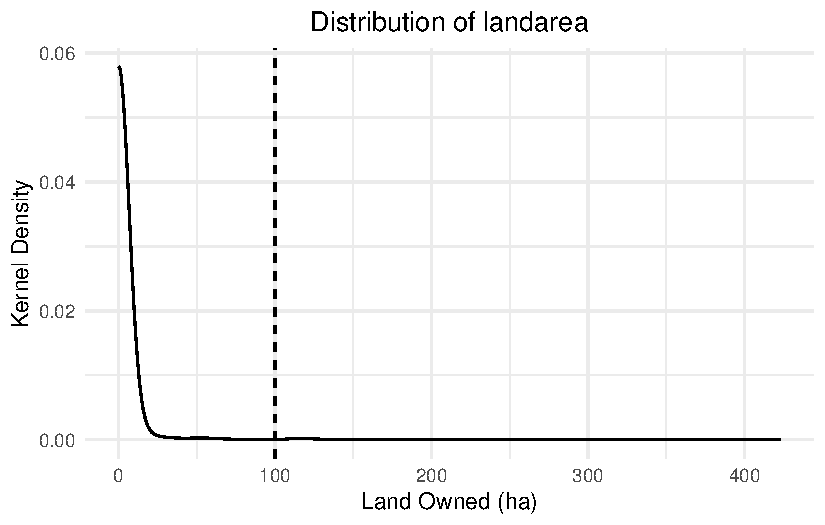
\includegraphics[keepaspectratio]{PS3_group1_files/figure-pdf/distribution_chart-1.pdf}}

 
\begin{table}[ht]
\begin{centerbox}
\begin{threeparttable}
\captionsetup{justification=centering,singlelinecheck=off}
\caption{Log-Linear model summary. Dependent variable: log(total household consumption).}
 \label{tbl-model_leq_100}\setlength{\tabcolsep}{0pt}
\begin{tabular}{l l l}


\hhline{>{\huxb{0, 0, 0}{0.8}}->{\huxb{0, 0, 0}{0.8}}->{\huxb{0, 0, 0}{0.8}}-}
\arrayrulecolor{black}

\multicolumn{1}{!{\huxvb{0, 0, 0}{0}}c!{\huxvb{0, 0, 0}{0}}}{\huxtpad{1.5pt + 1em}\centering \hspace{1.5pt}  \hspace{1.5pt}\huxbpad{1.5pt}} &
\multicolumn{1}{c!{\huxvb{0, 0, 0}{0}}}{\huxtpad{1.5pt + 1em}\centering \hspace{1.5pt} Base model \hspace{1.5pt}\huxbpad{1.5pt}} &
\multicolumn{1}{c!{\huxvb{0, 0, 0}{0}}}{\huxtpad{1.5pt + 1em}\centering \hspace{1.5pt} Land Area $<$= 100 \hspace{1.5pt}\huxbpad{1.5pt}} \tabularnewline[-0.5pt]


\hhline{>{\huxb{255, 255, 255}{0.4}}->{\huxb{0, 0, 0}{0.4}}->{\huxb{0, 0, 0}{0.4}}-}
\arrayrulecolor{black}

\multicolumn{1}{!{\huxvb{0, 0, 0}{0}}l!{\huxvb{0, 0, 0}{0}}}{\huxtpad{1.5pt + 1em}\raggedright \hspace{1.5pt} Intercept \hspace{1.5pt}\huxbpad{1.5pt}} &
\multicolumn{1}{r!{\huxvb{0, 0, 0}{0}}}{\huxtpad{1.5pt + 1em}\raggedleft \hspace{1.5pt} 9.178 *** \hspace{1.5pt}\huxbpad{1.5pt}} &
\multicolumn{1}{r!{\huxvb{0, 0, 0}{0}}}{\huxtpad{1.5pt + 1em}\raggedleft \hspace{1.5pt} 9.181 *** \hspace{1.5pt}\huxbpad{1.5pt}} \tabularnewline[-0.5pt]


\hhline{}
\arrayrulecolor{black}

\multicolumn{1}{!{\huxvb{0, 0, 0}{0}}l!{\huxvb{0, 0, 0}{0}}}{\huxtpad{1.5pt + 1em}\raggedright \hspace{1.5pt}  \hspace{1.5pt}\huxbpad{1.5pt}} &
\multicolumn{1}{r!{\huxvb{0, 0, 0}{0}}}{\huxtpad{1.5pt + 1em}\raggedleft \hspace{1.5pt} (0.108) \hspace{1.5pt}\huxbpad{1.5pt}} &
\multicolumn{1}{r!{\huxvb{0, 0, 0}{0}}}{\huxtpad{1.5pt + 1em}\raggedleft \hspace{1.5pt} (0.108) \hspace{1.5pt}\huxbpad{1.5pt}} \tabularnewline[-0.5pt]


\hhline{}
\arrayrulecolor{black}

\multicolumn{1}{!{\huxvb{0, 0, 0}{0}}l!{\huxvb{0, 0, 0}{0}}}{\huxtpad{1.5pt + 1em}\raggedright \hspace{1.5pt} Number of male adults \hspace{1.5pt}\huxbpad{1.5pt}} &
\multicolumn{1}{r!{\huxvb{0, 0, 0}{0}}}{\huxtpad{1.5pt + 1em}\raggedleft \hspace{1.5pt} 0.115 *** \hspace{1.5pt}\huxbpad{1.5pt}} &
\multicolumn{1}{r!{\huxvb{0, 0, 0}{0}}}{\huxtpad{1.5pt + 1em}\raggedleft \hspace{1.5pt} 0.114 *** \hspace{1.5pt}\huxbpad{1.5pt}} \tabularnewline[-0.5pt]


\hhline{}
\arrayrulecolor{black}

\multicolumn{1}{!{\huxvb{0, 0, 0}{0}}l!{\huxvb{0, 0, 0}{0}}}{\huxtpad{1.5pt + 1em}\raggedright \hspace{1.5pt}  \hspace{1.5pt}\huxbpad{1.5pt}} &
\multicolumn{1}{r!{\huxvb{0, 0, 0}{0}}}{\huxtpad{1.5pt + 1em}\raggedleft \hspace{1.5pt} (0.025) \hspace{1.5pt}\huxbpad{1.5pt}} &
\multicolumn{1}{r!{\huxvb{0, 0, 0}{0}}}{\huxtpad{1.5pt + 1em}\raggedleft \hspace{1.5pt} (0.025) \hspace{1.5pt}\huxbpad{1.5pt}} \tabularnewline[-0.5pt]


\hhline{}
\arrayrulecolor{black}

\multicolumn{1}{!{\huxvb{0, 0, 0}{0}}l!{\huxvb{0, 0, 0}{0}}}{\huxtpad{1.5pt + 1em}\raggedright \hspace{1.5pt} Number of female adults \hspace{1.5pt}\huxbpad{1.5pt}} &
\multicolumn{1}{r!{\huxvb{0, 0, 0}{0}}}{\huxtpad{1.5pt + 1em}\raggedleft \hspace{1.5pt} 0.195 *** \hspace{1.5pt}\huxbpad{1.5pt}} &
\multicolumn{1}{r!{\huxvb{0, 0, 0}{0}}}{\huxtpad{1.5pt + 1em}\raggedleft \hspace{1.5pt} 0.193 *** \hspace{1.5pt}\huxbpad{1.5pt}} \tabularnewline[-0.5pt]


\hhline{}
\arrayrulecolor{black}

\multicolumn{1}{!{\huxvb{0, 0, 0}{0}}l!{\huxvb{0, 0, 0}{0}}}{\huxtpad{1.5pt + 1em}\raggedright \hspace{1.5pt}  \hspace{1.5pt}\huxbpad{1.5pt}} &
\multicolumn{1}{r!{\huxvb{0, 0, 0}{0}}}{\huxtpad{1.5pt + 1em}\raggedleft \hspace{1.5pt} (0.025) \hspace{1.5pt}\huxbpad{1.5pt}} &
\multicolumn{1}{r!{\huxvb{0, 0, 0}{0}}}{\huxtpad{1.5pt + 1em}\raggedleft \hspace{1.5pt} (0.025) \hspace{1.5pt}\huxbpad{1.5pt}} \tabularnewline[-0.5pt]


\hhline{}
\arrayrulecolor{black}

\multicolumn{1}{!{\huxvb{0, 0, 0}{0}}l!{\huxvb{0, 0, 0}{0}}}{\huxtpad{1.5pt + 1em}\raggedright \hspace{1.5pt} Age of household head (years) \hspace{1.5pt}\huxbpad{1.5pt}} &
\multicolumn{1}{r!{\huxvb{0, 0, 0}{0}}}{\huxtpad{1.5pt + 1em}\raggedleft \hspace{1.5pt} 0.006 *** \hspace{1.5pt}\huxbpad{1.5pt}} &
\multicolumn{1}{r!{\huxvb{0, 0, 0}{0}}}{\huxtpad{1.5pt + 1em}\raggedleft \hspace{1.5pt} 0.006 *** \hspace{1.5pt}\huxbpad{1.5pt}} \tabularnewline[-0.5pt]


\hhline{}
\arrayrulecolor{black}

\multicolumn{1}{!{\huxvb{0, 0, 0}{0}}l!{\huxvb{0, 0, 0}{0}}}{\huxtpad{1.5pt + 1em}\raggedright \hspace{1.5pt}  \hspace{1.5pt}\huxbpad{1.5pt}} &
\multicolumn{1}{r!{\huxvb{0, 0, 0}{0}}}{\huxtpad{1.5pt + 1em}\raggedleft \hspace{1.5pt} (0.002) \hspace{1.5pt}\huxbpad{1.5pt}} &
\multicolumn{1}{r!{\huxvb{0, 0, 0}{0}}}{\huxtpad{1.5pt + 1em}\raggedleft \hspace{1.5pt} (0.002) \hspace{1.5pt}\huxbpad{1.5pt}} \tabularnewline[-0.5pt]


\hhline{}
\arrayrulecolor{black}

\multicolumn{1}{!{\huxvb{0, 0, 0}{0}}l!{\huxvb{0, 0, 0}{0}}}{\huxtpad{1.5pt + 1em}\raggedright \hspace{1.5pt} Education of household head (years) \hspace{1.5pt}\huxbpad{1.5pt}} &
\multicolumn{1}{r!{\huxvb{0, 0, 0}{0}}}{\huxtpad{1.5pt + 1em}\raggedleft \hspace{1.5pt} 0.066 *** \hspace{1.5pt}\huxbpad{1.5pt}} &
\multicolumn{1}{r!{\huxvb{0, 0, 0}{0}}}{\huxtpad{1.5pt + 1em}\raggedleft \hspace{1.5pt} 0.065 *** \hspace{1.5pt}\huxbpad{1.5pt}} \tabularnewline[-0.5pt]


\hhline{}
\arrayrulecolor{black}

\multicolumn{1}{!{\huxvb{0, 0, 0}{0}}l!{\huxvb{0, 0, 0}{0}}}{\huxtpad{1.5pt + 1em}\raggedright \hspace{1.5pt}  \hspace{1.5pt}\huxbpad{1.5pt}} &
\multicolumn{1}{r!{\huxvb{0, 0, 0}{0}}}{\huxtpad{1.5pt + 1em}\raggedleft \hspace{1.5pt} (0.005) \hspace{1.5pt}\huxbpad{1.5pt}} &
\multicolumn{1}{r!{\huxvb{0, 0, 0}{0}}}{\huxtpad{1.5pt + 1em}\raggedleft \hspace{1.5pt} (0.005) \hspace{1.5pt}\huxbpad{1.5pt}} \tabularnewline[-0.5pt]


\hhline{}
\arrayrulecolor{black}

\multicolumn{1}{!{\huxvb{0, 0, 0}{0}}l!{\huxvb{0, 0, 0}{0}}}{\huxtpad{1.5pt + 1em}\raggedright \hspace{1.5pt} Land owned (ha) \hspace{1.5pt}\huxbpad{1.5pt}} &
\multicolumn{1}{r!{\huxvb{0, 0, 0}{0}}}{\huxtpad{1.5pt + 1em}\raggedleft \hspace{1.5pt} 0.004 *** \hspace{1.5pt}\huxbpad{1.5pt}} &
\multicolumn{1}{r!{\huxvb{0, 0, 0}{0}}}{\huxtpad{1.5pt + 1em}\raggedleft \hspace{1.5pt} 0.010 ** \hspace{1.5pt}\huxbpad{1.5pt}} \tabularnewline[-0.5pt]


\hhline{}
\arrayrulecolor{black}

\multicolumn{1}{!{\huxvb{0, 0, 0}{0}}l!{\huxvb{0, 0, 0}{0}}}{\huxtpad{1.5pt + 1em}\raggedright \hspace{1.5pt}  \hspace{1.5pt}\huxbpad{1.5pt}} &
\multicolumn{1}{r!{\huxvb{0, 0, 0}{0}}}{\huxtpad{1.5pt + 1em}\raggedleft \hspace{1.5pt} (0.001) \hspace{1.5pt}\huxbpad{1.5pt}} &
\multicolumn{1}{r!{\huxvb{0, 0, 0}{0}}}{\huxtpad{1.5pt + 1em}\raggedleft \hspace{1.5pt} (0.004) \hspace{1.5pt}\huxbpad{1.5pt}} \tabularnewline[-0.5pt]


\hhline{}
\arrayrulecolor{black}

\multicolumn{1}{!{\huxvb{0, 0, 0}{0}}l!{\huxvb{0, 0, 0}{0}}}{\huxtpad{1.5pt + 1em}\raggedright \hspace{1.5pt} Distance to health centre (km) \hspace{1.5pt}\huxbpad{1.5pt}} &
\multicolumn{1}{r!{\huxvb{0, 0, 0}{0}}}{\huxtpad{1.5pt + 1em}\raggedleft \hspace{1.5pt} -0.011 \hspace{1.5pt}\huxbpad{1.5pt}} &
\multicolumn{1}{r!{\huxvb{0, 0, 0}{0}}}{\huxtpad{1.5pt + 1em}\raggedleft \hspace{1.5pt} -0.010 \hspace{1.5pt}\huxbpad{1.5pt}} \tabularnewline[-0.5pt]


\hhline{}
\arrayrulecolor{black}

\multicolumn{1}{!{\huxvb{0, 0, 0}{0}}l!{\huxvb{0, 0, 0}{0}}}{\huxtpad{1.5pt + 1em}\raggedright \hspace{1.5pt}  \hspace{1.5pt}\huxbpad{1.5pt}} &
\multicolumn{1}{r!{\huxvb{0, 0, 0}{0}}}{\huxtpad{1.5pt + 1em}\raggedleft \hspace{1.5pt} (0.010) \hspace{1.5pt}\huxbpad{1.5pt}} &
\multicolumn{1}{r!{\huxvb{0, 0, 0}{0}}}{\huxtpad{1.5pt + 1em}\raggedleft \hspace{1.5pt} (0.011) \hspace{1.5pt}\huxbpad{1.5pt}} \tabularnewline[-0.5pt]


\hhline{}
\arrayrulecolor{black}

\multicolumn{1}{!{\huxvb{0, 0, 0}{0}}l!{\huxvb{0, 0, 0}{0}}}{\huxtpad{1.5pt + 1em}\raggedright \hspace{1.5pt} Distance to school (km) \hspace{1.5pt}\huxbpad{1.5pt}} &
\multicolumn{1}{r!{\huxvb{0, 0, 0}{0}}}{\huxtpad{1.5pt + 1em}\raggedleft \hspace{1.5pt} -0.020 * \hspace{1.5pt}\huxbpad{1.5pt}} &
\multicolumn{1}{r!{\huxvb{0, 0, 0}{0}}}{\huxtpad{1.5pt + 1em}\raggedleft \hspace{1.5pt} -0.020 * \hspace{1.5pt}\huxbpad{1.5pt}} \tabularnewline[-0.5pt]


\hhline{}
\arrayrulecolor{black}

\multicolumn{1}{!{\huxvb{0, 0, 0}{0}}l!{\huxvb{0, 0, 0}{0}}}{\huxtpad{1.5pt + 1em}\raggedright \hspace{1.5pt}  \hspace{1.5pt}\huxbpad{1.5pt}} &
\multicolumn{1}{r!{\huxvb{0, 0, 0}{0}}}{\huxtpad{1.5pt + 1em}\raggedleft \hspace{1.5pt} (0.011) \hspace{1.5pt}\huxbpad{1.5pt}} &
\multicolumn{1}{r!{\huxvb{0, 0, 0}{0}}}{\huxtpad{1.5pt + 1em}\raggedleft \hspace{1.5pt} (0.011) \hspace{1.5pt}\huxbpad{1.5pt}} \tabularnewline[-0.5pt]


\hhline{>{\huxb{255, 255, 255}{0.4}}->{\huxb{0, 0, 0}{0.4}}->{\huxb{0, 0, 0}{0.4}}-}
\arrayrulecolor{black}

\multicolumn{1}{!{\huxvb{0, 0, 0}{0}}l!{\huxvb{0, 0, 0}{0}}}{\huxtpad{1.5pt + 1em}\raggedright \hspace{1.5pt} N \hspace{1.5pt}\huxbpad{1.5pt}} &
\multicolumn{1}{r!{\huxvb{0, 0, 0}{0}}}{\huxtpad{1.5pt + 1em}\raggedleft \hspace{1.5pt} 575 \hspace{1.5pt}\huxbpad{1.5pt}} &
\multicolumn{1}{r!{\huxvb{0, 0, 0}{0}}}{\huxtpad{1.5pt + 1em}\raggedleft \hspace{1.5pt} 569 \hspace{1.5pt}\huxbpad{1.5pt}} \tabularnewline[-0.5pt]


\hhline{}
\arrayrulecolor{black}

\multicolumn{1}{!{\huxvb{0, 0, 0}{0}}l!{\huxvb{0, 0, 0}{0}}}{\huxtpad{1.5pt + 1em}\raggedright \hspace{1.5pt} R2 \hspace{1.5pt}\huxbpad{1.5pt}} &
\multicolumn{1}{r!{\huxvb{0, 0, 0}{0}}}{\huxtpad{1.5pt + 1em}\raggedleft \hspace{1.5pt} 0.354 \hspace{1.5pt}\huxbpad{1.5pt}} &
\multicolumn{1}{r!{\huxvb{0, 0, 0}{0}}}{\huxtpad{1.5pt + 1em}\raggedleft \hspace{1.5pt} 0.336 \hspace{1.5pt}\huxbpad{1.5pt}} \tabularnewline[-0.5pt]


\hhline{>{\huxb{0, 0, 0}{0.8}}->{\huxb{0, 0, 0}{0.8}}->{\huxb{0, 0, 0}{0.8}}-}
\arrayrulecolor{black}
\end{tabular}
\begin{tablenotes}[flushleft]
\item[] Significance: *** p $<$ 0.01; ** p $<$ 0.05; * p $<$ 0.1
\end{tablenotes}
\end{threeparttable}\par\end{centerbox}

\end{table}
 

\begin{center}\rule{0.5\linewidth}{0.5pt}\end{center}

\subsection{Question (7): Omitted Variable Thought
Experiment}\label{question-7-omitted-variable-thought-experiment}

\emph{Give an example of an additional variable you might want to
include in the regression, but for which you don't have data, and
indicate the expected effect of that variable, as well as any changes
you would anticipate to occur in the point estimates of the other
variables.}

\begin{tcolorbox}[enhanced jigsaw, arc=.35mm, bottomrule=.15mm, bottomtitle=1mm, breakable, colback=white, colbacktitle=quarto-callout-note-color!10!white, colframe=quarto-callout-note-color-frame, coltitle=black, left=2mm, leftrule=.75mm, opacityback=0, opacitybacktitle=0.6, rightrule=.15mm, title=\textcolor{quarto-callout-note-color}{\faInfo}\hspace{0.5em}{Answer --- Question (7)}, titlerule=0mm, toprule=.15mm, toptitle=1mm]

\end{tcolorbox}




\end{document}
